\documentclass[11pt, norsk]{article}
%\usepackage[latin1]{inputenc}
\usepackage[T1]{fontenc}
\usepackage[utf8]{inputenc}
\usepackage[norsk]{babel}   % S P R A A K


% \usepackage{graphicx}    % postscript graphics
\usepackage{amssymb, amsmath, amsthm, amssymb} % symboler, osv
\usepackage{mathrsfs}
\usepackage{url}
\usepackage{thmtools}
\usepackage{enumerate}  % lister $  
\usepackage{float}
\usepackage{tikz}
\usetikzlibrary{calc}
\usetikzlibrary{intersections}
\usepackage{tikz-3dplot}
\usepackage{subcaption}
\usepackage[all]{xy}   % for comm.diagram
\usepackage{wrapfig} % for float right
\usepackage{hyperref}
\usepackage{mystyle} % stilfilen      


\begin{document}
\title{Oppgaver MAT2500}
\author{Fredrik Meyer}
\maketitle 

\begin{oppg}
Finn sentrum og halvakser til kjeglesnittet med ligningen $$25x^2+ 9y^2-18x+2y=0.$$
\end{oppg}
\begin{losn}
Vi vet at alle ikke degenererte kjeglesnitt er enten ellipser, hyperbler eller parabler. Siden det er snakk om "halvakser", regner vi kanskje med at dette blir en ellipse. For å finne sentrum er det ikke annet å gjøre enn å begynne å fullføre kvadrater. Vi tar $x$- og $y$-leddene hver for seg.

\begin{align*}
25x^2-18x &= (5x)^2-2 \cdot (5x) \cdot \frac{9}{5} \\
&= (5x)^2 - 2 \cdot (5x) \cdot \frac 95 + \frac{81}{25} - \frac{81}{25} \\
&= (5x - \frac 95)^2 - \frac{81}{25}.
\end{align*}

Og tilsvarende for $y$ finner vi at
$$
9y^2+2y = (3y+\frac 13)^2- \frac 49.
$$

Dermed finner vi at kjeglesnittet kan skrives som 
$$
(5x-\frac 95)^2 + (3y + \frac 13)^2 = \frac{754}{225}.
$$
Vi ser med en gang at dette er en ellipse. Men standardligningen for en ellipse ser ut som $x^2/a^2+y^2/b^2=1$, så må må dele på høyresiden og ta ut konstantene fra leddene. Vi får 
$$
\frac{\left(x-\frac{9}{25}\right)^2}{\left(\frac{\sqrt{754}}{225}\right)^2} + 
\frac{\left(y-\frac{1}{9}\right)^2}{\left(\frac{\sqrt{754}}{45}\right)^2} = 0
$$
Da er sentrum $(\frac 9{25},\frac 19)$, og halvaksene er nevnerne.
\end{losn}

\begin{oppg}
Finn asymptoter og eksentrisitet til hyperbelen med ligning
$$
9x^2-4y^2-18x+4y-6=0.
$$
\end{oppg}
\begin{losn}
Det er bare å fullføre kvadrater. Her tar jeg ikke med utregningen. Vi ender opp med 
$$
\frac{\left(x-1\right)^2}{\frac {14}9} - \frac{\left(y-\frac 12\right)^2}{\frac{14}{4}} = 1.
$$
Dermed er $a= \sqrt{14}/3$ og $b=\sqrt{14}/2$. Eksentrisiteten er definert som $c/a$ der $c$ tilfredsstiller $a^2+b^2=c^2$. Vi finner at $c=\sqrt{91/18}$. Dermed er eksentrisiteten $e=\sqrt{13}/2$.

Asymptotene er $y=\frac {3x}2 -1$ og $y = -\frac{3x}{2} +2$.
\end{losn}

\begin{oppg}
Finn ligningen og symmetriaksene til det geometriske stedet for punkter som har dobbelt så stor avstand til punktet $(1,2)$ som til linja $y=5$.
\end{oppg}
\begin{losn}
Skriv $P=(x,y)$. Da er betingelsen vår at $$\lvert (x-1,y-2) \rvert = 2 \lvert y - 5 \rvert.$$

Vi kvadrerer begge sider, og fullfører kvadrater som før. Vi får en hyperbel gitt ved ligningen
$$
\frac{\left( y- 6 \right)^2}{4} - \frac{\left(x-1\right)^2}{12} = 1.
$$
Symmetriaksene blir da gitt ved $y=6$ og $x=1$. Se Figur 1.
\begin{figure}
\begin{tikzpicture}
 \draw[->] (-3,0) -- (7,0);
  \draw[->] (0,-1) -- (0,9);
    \pgfmathsetmacro{\e}{2}   % eccentricity
    \pgfmathsetmacro{\a}{2}
    \pgfmathsetmacro{\b}{(\a*sqrt((\e)^2-1)} 
    \draw plot[domain=-1.3:1.3] ({\b*sinh(\x)+1},{\a*cosh(\x)+6});
    \draw plot[domain=-1.3:1.3] ({\b*sinh(\x)+1},{-\a*cosh(\x)+6});
    \fill[black] (1,2) circle (2.0pt);
    \draw (1.2,2.2) node {P};
    \draw[thick] (-5,5) -- (7,5) node[above] {$y=5$};
\end{tikzpicture}
\caption{Oppgave 3.}
\end{figure}
\end{losn}

\begin{oppg}
Finn brennpunkt og styrelinje for parabelen $y=x^2$. Finn det geometriske stedet for midtpunktet til kordene til parabelen som går gjennom brennpunktet.
\end{oppg}
\begin{losn}
Ved å se i tabellen, eventuelt tenke selv, ser vi at brennpunktet er gitt ved $(0,\frac 14)$ og styrelinja er gitt ved $y=-\frac 14$.

Vi ønsker å finne et uttrykk for midtpunktet til en korde gjennom brennpunktet slik at vi får alle slike midtpunkter.

La $y=ax+b$. Vi ønsker at linja $y(x)$ skal gå gjennom brennpunktet til parabelen. Dette er det samme som å kreve at $y(0)=\frac 14=b$. Dermed er en generell linje som går gjennom brennpunktet gitt ved $y=ax+\frac 14$, og vi får alle slike linjer ved å la $a$ variere.

Neste steg er å finne midtpunktet på korden linja definerer. For å finne det, trenger vi skjæringspunktene med linja. Vi setter ligninga for linja inn i $y= x^2$, og får andregradsligningen $$x^2-ax-\frac 14=0.$$

Her er en generell observasjon: om en andregradsligning $x^2+bx+c=0$ har røttene $x_1$ og $x_2$, så er $x^2+bx+c=(x-x_1)(x-x_2)=x^2-(x_1+x_2)x+x_1x_2=0$. Dermed ser vi at $b=-x_1-x_2$.

I vårt tilfelle ser vi at midtpunktet har $x$-koordinat $\frac a2$. Ved å bruke at $y=ax+b$, får vi at $y$-koordinaten er gitt ved $\frac {a^2}{2}+\frac 14$. 

Dermed er alle midtpunkter gitt ved
$$\left( \frac a2 , \frac {a^2}{2}+\frac 14 \right) $$
når $a$ varierer. Sett $a' = \frac a2$. Da blir uttrykket over lik
$$\left( a', 2{a'}^2+\frac 14 \right) .$$
Dermed er det geometriske stedet gitt ved ligningen $y = 2x^2+\frac 14$. 
\end{losn}

\begin{oppg}
La $A$ være et punkt på parabelen $x=y^2$ og la $B$ være det andre punktet på parabelen som har samme $x$-koordinat som $A$. La $P$ være skjæringspunktet mellom tangentlinja til parabelen i $A$ og linja gjennom origo og $B$. Finn ligningen til det geometriske stedet for $P$ når $A$ gjennomløper parabelen.
\end{oppg}
\begin{losn}
La $A=(b^2,b)$ for $b \in \R$. Da er $B=(b^2,-b)$. 

Første steg er å finne ligningene for de to linjene. Man kan regne ut at, for eksempel med implisitt derivasjon, at stigningstallet til linja gjennom $A$ er $\frac{1}{2b}$. Dermed finner vi at linja er gitt ved $y = \frac{1}{2b}x + \frac{b}{2}$. 

Linja gjennom $B$ og origo er gitt ved $y= - \frac{x}{b}$.

Skjæringspunktet mellom disse linjene blir da gitt ved (etter litt regning) $\left( - \frac{b^2}{3}, \frac b3 \right)$. Setter vi $b' = \frac b3$, får vi at skjæringspunktet kan skrives som $ (-3{b'}^2,b')$, så det geometriske stedet er parabelen gitt ved $x= 3y^2$.
\end{losn}

\begin{oppg}
La $\ell_1$ og $\ell_2$ være gitt ved
$$
x + 3y+4=0 \qquad \text{og} \qquad x+3y-4=0.
$$
La $\ell$ være ei linje gjennom origo som skjæren den første linja i $A$ og den andre i $B$. Trekk en linje gjennom $A$ parallell med $y$-aksen og gjennom $B$ parallell med $x$-aksen. Finn det geometriske stedet for skjæringspunktet mellom disse parallellene når $l$ dreier seg om origo.
\end{oppg}

\begin{losn}
Dette er stort sett samme framgangsmåte som forrige oppgave, så jeg skisserer bare en løsning.

Om vi lar linja gjennom origo være definert ved $y=ax$, finner vi at $A$ og $B$ er gitt ved (henholdsvis):
$$
\left( \frac{-4}{1+3a}, \frac{-4a}{1+3a} \right) \qquad \text{og} \qquad 
\left( \frac{4}{1+3a}, \frac{4a}{1+3a} \right).
$$
Dermed er de parallelle linjene gitt ved 
$$
y = \frac{-4a}{1+4a} \qquad \text{og} \qquad x = \frac{4}{1+3a}.
$$
Så skjæringspunktet er
$$
P = \left(\frac{4}{1+4a}, \frac{-4a}{1+4a} \right).
$$
Setter vi $a' = \frac{4}{1+3a}$, får vi, på samme måte som de andre oppgavene, at det geometriske stedet er gitt ved ligningen $y = \frac{-4+a'}{3}$, som er en linje.
\end{losn}

\begin{oppg}
En sirkel med sentrum i origo skjærer $x$-aksen i $A=(-r,0)$ og $B=(r,0)$. La $M$ være midtpunktet på normalen fra et punkt $P$ på sirkelen på $x$-aksen. Finn det geometriske stedet for skjæringspunktet mellom $AP$ og $BM$ når $P$ beveger seg på sirkelen.
\end{oppg}

\begin{losn}
Se Figur 2. Igjen: jeg skisserer løsningen, og lar noen andre gjøre all regningen. Første steg er å finne koordinatene til alle punktene. Om $P=(x,y)$, så er $M=(x,\frac 12 y)$.

Man finner så ligningen for linja gjennom $(r,0)$ og $(x,\frac 12y)$. Og også ligningen for linja mellom $(-r,0)$ og $(x,y)$. Man regner så ut skjæringspunktet mellom disse.

Her er det viktig å gjøre ting sakte og oversiktlig, for det blir fort ganske stygge utregninger. 

Man finner så at $S$ ser ut som

$$
\left(r \frac{3x-1}{3-x}, r \frac{2y}{3-x}\right).
$$

Ved å kvadrere $x$-koordinaten og $y$-koordinaten og legge sammen, og å bruke at $x^2+y^2=r^2$, kan dette skrives om til ligningen for en ellipse.

Vi skal ende opp med en ellipse med ligning $x^2 + \frac{y^2}{1/2} = r^2$.
\begin{figure}
\begin{center}
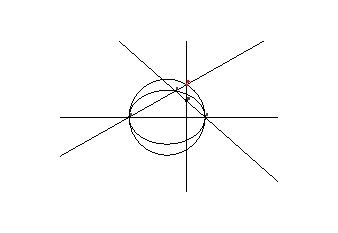
\includegraphics[scale=3.5]{mat2500oppg9bilde}
\caption{Figur 2.}
\end{center}
\end{figure}
\end{losn}






\end{document}
